\documentclass{beamer}

\usetheme{Berlin}

\usecolortheme{dolphin}

\usepackage{amsmath}
\usepackage{graphicx}
\usepackage{setspace}
\usepackage{animate}

\newcommand{\abs}[1]{\left \vert #1 \right \vert}
\newcommand{\norm}[1]{\left \Vert #1 \right \Vert}
\newcommand{\order}[1]{\mathcal{O} \left ( #1 \right )}
\newcommand{\set}[1]{\left \{ #1 \right \}}
\newcommand{\Set}[2]{\left \{ #1 \middle \vert #2 \right \}}

\newcommand{\inner}[2]{\left \langle #1, #2 \right \rangle}

\title{Introduction to Spectral Collocation}
\author{Conor McCoid}
\institute{University of Geneva}
\date{April 8th, 2019}

\begin{document}

\frame{\titlepage}

\begin{frame}

\begin{block}{The continuous problem}
$\mathcal{L} u(x) = f(x)$
\end{block}

\begin{description}
\item[$\mathcal{L}$:] Some linear operator acting on the function $u(x)$
\item[$u(x)$:] Some real-valued function (with some regularity) acting on a point $x \in \Omega \subset \mathbb{R}$
\item[$f(x)$:] Some real-valued function (with possibly different regularity than $u(x)$) acting on the same point $x$
\end{description}

\end{frame}

\begin{frame}

\begin{block}{The discrete problem}
$L_N u_N = f_N$
\end{block}

\begin{description}
\item[$L_N$:] Some operator taking $N$ pieces of information from $u_N$ and returning $N$ pieces of information in $f_N$, ie. $L_N : \mathbb{R}^N \rightarrow \mathbb{R}^N$
\item[$u_N$:] Some set of $N$ pieces of information, ie. $u_N \in \mathbb{R}^N$
\item[$f_N$:] Some set of $N$ pieces of information, ie. $f_N \in \mathbb{R}^N$
\end{description}

\end{frame}

\begin{frame}

By the description of the discrete problem $L_N$ is some matrix of size $N \times N$ and $u_N$ and $f_N$ are both vectors of length $N$.
The solution vector $u_N$ is then $u_N = L_N^{-1} f_N$.

~

We want our solution vector $u_N$ to correspond in some way to the solution function of the continuous problem.
That is, we want
\begin{equation*}
\lim_{N \to \infty} u_N \equiv u(x)
\end{equation*}
in some sense.

% At this stage it would be helpful to draw a diagram, showing the discrete spaces inside the continuous ones and how the projection would work
\end{frame}

\begin{frame}

The discrete space may be defined by a set of basis functions (called \textit{trial functions}), $\set{\phi_k(x)}_{k=1}^N$.
Our approximation $u_N$ then defines a linear combination of these functions:
\begin{equation*}
u_N \equiv \sum_{k=1}^N a_k \phi_k(x) .
\end{equation*}

\end{frame}

\begin{frame}

We want now that when we apply $\mathcal{L}$ to this linear combination, we'll retrieve an approximation to $f(x)$:
\begin{equation*}
\sum_{k=1}^N a_k \mathcal{L} \phi_k(x) \approx f(x) .
\end{equation*}
More specifically, we want that
\begin{equation*}
\inner{\sum_{k=1}^N a_k \mathcal{L} \phi_k(x) - f(x) }{\psi_j(x) } = 0 \ \forall j=1,...,N
\end{equation*}
for some inner product defined on the space of functions and for some set of \textit{test functions} $\psi_j(x)$.

\end{frame}

\begin{frame}
This allows us to choose three things:
\begin{itemize}
\item the inner product $\inner{\cdot}{\cdot}$,
\item the trial functions $\phi_k(x)$,
\item and the test functions $\psi_j(x)$.
\end{itemize}

Different sets of these choices lead to different classes of methods.
\end{frame}

\begin{frame}

\begin{block}{Finite Element Methods}
$\phi_k(x)$ and $\psi_j(x)$ have finite support (locally defined).
\end{block}
~
\begin{block}{Spectral Methods}
$\phi_k(x)$ and $\psi_j(x)$ have infinite support (globally defined).
\end{block}
% main difference, not only difference
\end{frame}

\begin{frame}

\begin{block}{Galerkin}
The trial functions individually satisfy the boundary conditions.
\end{block}

\begin{block}{Tau} % I don't think this is right
$\inner{\phi_k(x)}{\psi_j(x)} = \begin{cases} 1 & k = j \\ 0 & k \neq j \end{cases} $
\end{block}

\begin{block}{Collocation}
$\inner{\phi_k(x)}{\psi_j(x)} = \phi_k(x_j)$
\end{block}
% not exactly their definitions but they'll give us the right idea
\end{frame}

\begin{frame}
\begin{description}
\item[Galerkin] $u_N$ contains the coefficients in the \textit{Galerkin basis}.
\item[Tau] $u_N$ also contains coefficients, but for a more general basis.
\item[Collocation] $u_N$ contains the values of the approximation at some set of \textit{collocation points}, $u_N(x_j)$.
\end{description}
\end{frame}

\begin{frame}

We will focus on spectral collocation (global basis functions, minimize residual point by point).
That is,
\begin{equation*}
L_N \begin{bmatrix}
u_N(x_1) \\ u_N(x_2) \\ \vdots \\ u_N(x_N)
\end{bmatrix} = \begin{bmatrix}
f(x_1) \\ f(x_2) \\ \vdots \\ f(x_N)
\end{bmatrix}
\end{equation*}
with $L_N$ being a matrix representing the linear operator.

~

We need to know $L_N$ to solve this system.
For that, we need to know the differentiation matrix, $D_N$.

\end{frame}

\begin{frame}

$D_N$ must work perfectly for the trial functions, $\phi_k(x)$:
\begin{equation*}
D_N \begin{bmatrix}
\phi_k(x_1) \\ \phi_k(x_2) \\ \vdots \\ \phi_k(x_N)
\end{bmatrix} = \begin{bmatrix}
\phi_k'(x_1) \\ \phi_k'(x_2) \\ \vdots \\ \phi_k'(x_N)
\end{bmatrix}
\end{equation*}
for all $k = 1,...,N$.

~

$D_N$ is singular since $D_N \begin{bmatrix} 1 & 1 & \dots & 1 \end{bmatrix}^\top = 0$ (nilpotent, actually).
The matrix representing second order differentiation is the square of $D_N$.
Likewise, $D^{(m)}_N = D^m_N$.
% you can think of D_N like you would a finite difference matrix: it performs differentiation on functions defined on a given set of points
\end{frame}

\begin{frame}

\begin{block}{The continuous operator}
\begin{equation*}
\mathcal{L} u(x) = u^{(m)}(x) + \sum_{k=1}^m p_k(x) u^{(m-k)}(x)
\end{equation*}
\end{block}
\begin{block}{The discrete operator}
\begin{equation*}
L_N = D^m_N + \sum_{k=1}^m P_k D^{m-k}_N
\end{equation*}
where $P_k$ is a $N \times N$ diagonal matrix with entries $p_k(x_j)$.
\end{block}

\end{frame}

\begin{frame}
$L_N$ is singular because $D_N$ and all of its powers are singular.
Boundary conditions are needed to make $L_N$ nonsingular.
The number of BCs matches the order of the problem, $m$.

~

BCs may be concatenated so the system is overdetermined or they can be used to replace rows in $L_N$.
\end{frame}

\begin{frame}

What should we choose for $\phi_k(x)$?
\begin{itemize}
\item $\phi_k(x)$ span a finite dimensional space
\item they should be orthogonal with respect to some inner product (generally a weighted $L_2$ inner product)
\item they can be used to approximate functions in the infinite space arbitrarily well
\end{itemize}

Some candidates:
\begin{itemize}
\item Sinusoids (Fourier series)
\item Polynomials (Weierstrass approximation theorem)
\end{itemize}

\end{frame}

\begin{frame}

\frametitle{Jacobi polynomials}

\begin{align*}
& P_n^{(\alpha, \beta)}(x) = \\
& \frac{\Gamma(\alpha + n + 1)}{n! \Gamma(\alpha + \beta + n + 1)} \sum_{m=0}^n \binom{n}{m} \frac{\Gamma(\alpha + \beta + n + m + 1)}{\Gamma(\alpha + m + 1)} \left ( \frac{x-1}{2} \right )^m
\end{align*}

Orthogonal with respect to the weight $(1-x)^\alpha (1+x)^\beta$ on $[-1,1]$

\end{frame}

\begin{frame}

\frametitle{Ultraspherical polynomials}

Special cases of the Jacobi polynomials with $\alpha = \beta$

\begin{block}{Legendre polynomials}
$\alpha = \beta = 0$
\end{block}

\begin{block}{Chebyshev polynomials}
$\alpha = \beta = 1/2$
\end{block}

\end{frame}

\begin{frame}

\frametitle{Sturm-Liouville Theory}

The Sturm-Liouville Problem (SLP):
\begin{equation*}
\mathcal{L}_{SL} \phi(x) = -\left ( p(x) \phi'(x) \right )' + q(x) \phi(x) = \lambda w(x) \phi(x)
\end{equation*}
with $p \in C^1(-1,1)$, $p>0$, $q, w \geq 0$, $q, w \in C[-1,1]$.

~

If $\mathcal{L}_{SL}$ is self-adjoint ($\inner{\mathcal{L}_{SP}u}{v} = \inner{u}{\mathcal{L}_{SP}v}$) then the SLP has a countable number of eigenvalues ($\lambda$) and the eigenfunctions ($\phi(x)$) form a complete set in $L^2(-1,1)$ and $L_w^2(-1,1) = \Set{u \in L^2(-1,1)}{\int_{-1}^1 u^2 w dx < \infty}$.
% in essence, the functions phi(x) make great candidates for our basis functions
\end{frame}

\begin{frame}

The projection of a function $u(x) \in L_w^2(-1,1)$ onto a finite space spanned by the first $N$ eigenfunctions may be written as
\begin{equation*}
P_N u(x) = \sum_{k=1}^N \hat{u}_k \phi_k(x)
\end{equation*}
where $\hat{u}_k = \int_{-1}^1 \phi_k(x) u(x) w(x) dx / \lambda_k$.

~

If $p(\pm 1) = 0$ and $u \in C^\infty(-1,1)$ then $\abs{\hat{u}_k} \to 0$ faster than any polynomial power of $1/k$ (known as spectral convergence).

\end{frame}

\begin{frame}

Special cases of SLP: ultraspherical polynomials
\begin{itemize}
\item $p(x) = (1-x^2)^{\alpha+1}$
\item $q(x) =c(1-x^2)^\alpha$
\item $w(x) = (1-x^2)^\alpha$
\end{itemize}
For $\alpha = 0$ the eigenfunctions are the Legendre polynomials.
For $\alpha = 1$ the eigenfunctions are the Chebyshev polynomials.

\end{frame}

\begin{frame}

\frametitle{Legendre polynomials}

\begin{block}{Rodrigues' formula}
\begin{equation*}
P_n(x) = \frac{1}{2^n n!} \frac{d^n}{dx^n} (x^2-1)^n
\end{equation*}
\end{block}

\begin{figure}
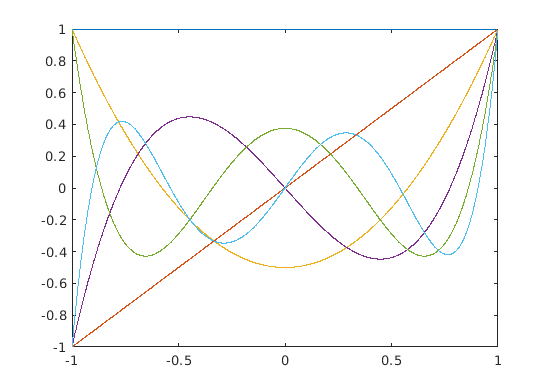
\includegraphics[width=0.5\textwidth]{legendreP.png}
\end{figure}

\end{frame}

\begin{frame}

\frametitle{Chebyshev polynomials}

\begin{block}{Closed form}
\begin{equation*}
T_n(x) = \cos \left ( n \arccos \left ( x \right ) \right )
\end{equation*}
\end{block}

\begin{figure}
\includegraphics[width=0.5\textwidth]{chebyshevT.png}
\end{figure}

\end{frame}

\end{document}